\documentclass[tikz,border=12pt]{standalone}
\usepackage{amsmath,amssymb}
\usetikzlibrary{calc,arrows.meta}

\begin{document}
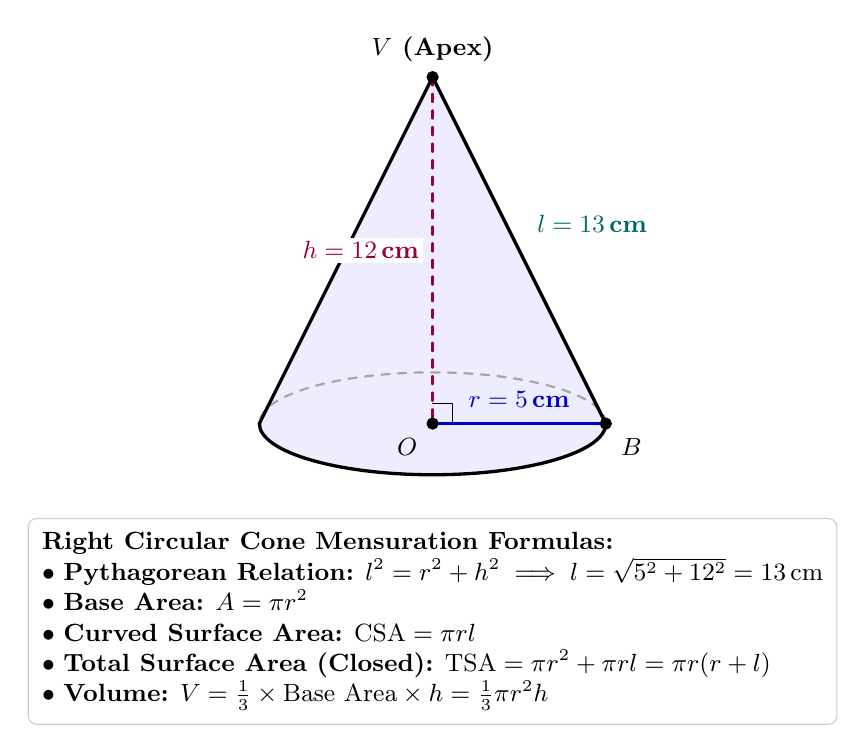
\begin{tikzpicture}[>=latex, line cap=round, line join=round]

  % Dimensions (proportions: rx = 2.2, ry = 0.65, height h = 4.4)
  \def\rx{2.2}
  \def\ry{0.65}
  \def\h{4.4}

  % Cone lateral body shading
  \fill[blue!7] (-\rx, 0) arc (180:360:\rx cm and \ry cm) -- (0, \h) -- cycle;

  % Hidden back half of base ellipse (dashed)
  \draw[thick, dashed, gray!70] (\rx, 0) arc (0:180:\rx cm and \ry cm);

  % Visible front half of base ellipse (solid)
  \draw[very thick] (-\rx, 0) arc (180:360:\rx cm and \ry cm);

  % Lateral contours
  \draw[very thick] (-\rx, 0) -- (0, \h);
  \draw[very thick] (\rx, 0) -- (0, \h);

  % Internal right triangle V-O-B:
  % Vertical altitude (dashed)
  \draw[thick, dashed, purple!80!black] (0, \h) -- (0, 0) node[midway, left=3pt, font=\small\bfseries, fill=white, inner sep=1.5pt] {$h = 12\,\text{cm}$};

  % Horizontal base radius (solid, label above to avoid base arc)
  \draw[thick, blue!80!black] (0, 0) -- (\rx, 0) node[midway, above=2pt, font=\small\bfseries] {$r = 5\,\text{cm}$};

  % Slant height callout on right contour
  \path (0, \h) -- (\rx, 0) node[midway, above right=3pt, font=\small\bfseries, teal!80!black] {$l = 13\,\text{cm}$};

  % Right angle indicator at center O
  \draw[thin] (0, 0.25) -- (0.25, 0.25) -- (0.25, 0);

  % Points
  \filldraw[black] (0, \h) circle (2pt) node[above=2pt, font=\small\bfseries] {$V$ (Apex)};
  \filldraw[black] (0, 0) circle (2pt) node[below left=2pt, font=\small\bfseries] {$O$};
  \filldraw[black] (\rx, 0) circle (2pt) node[below right=2pt, font=\small\bfseries] {$B$};

  % Formula Card below
  \node[align=left, font=\small, fill=white, inner sep=5pt, draw=gray!40, rounded corners=3pt, anchor=north] at (0, -1.2) {
    \textbf{Right Circular Cone Mensuration Formulas:}\\
    $\bullet$ \textbf{Pythagorean Relation:} $l^2 = r^2 + h^2 \implies l = \sqrt{5^2 + 12^2} = 13\,\text{cm}$\\
    $\bullet$ \textbf{Base Area:} $A = \pi r^2$\\
    $\bullet$ \textbf{Curved Surface Area:} $\text{CSA} = \pi r l$\\
    $\bullet$ \textbf{Total Surface Area (Closed):} $\text{TSA} = \pi r^2 + \pi r l = \pi r(r + l)$\\
    $\bullet$ \textbf{Volume:} $V = \frac{1}{3} \times \text{Base Area} \times h = \frac{1}{3}\pi r^2 h$
  };

\end{tikzpicture}
\end{document}
